\section{Solution}
\subsection{Naive Priority}

\begin{frame}{Naive Priority}
  \begin{itemize}
    \item Assign priority to conflicting requests
    \item User needs to specify the order to provide deterministic results and resolve concurrent conflict
    \item Challenge: Naive scheme that assumes user can predict all possible combination that may happen for specific application
  \end{itemize}
  \end{frame}

\begin{frame}
	Conflict in K-cluster
			\begin{figure}
			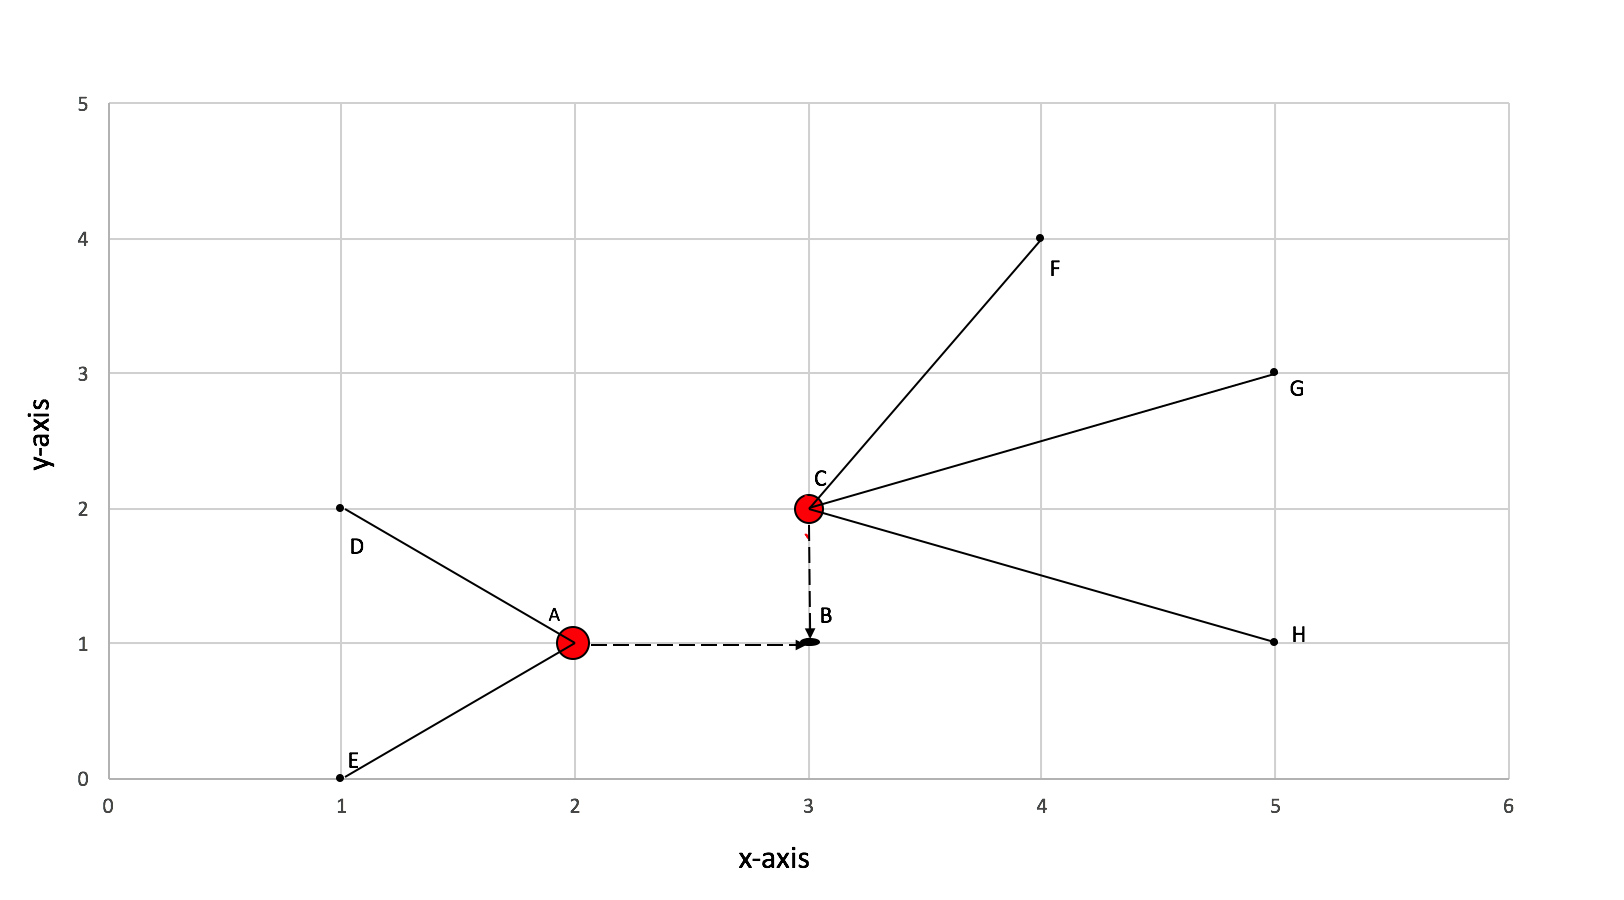
\includegraphics[width=0.6\linewidth]{figures/priority2.png}
			\caption{Solution Using Priority Models}
			\end{figure}
\end{frame}

\begin{frame}
	Conflict in dangling edge
			\begin{figure}
			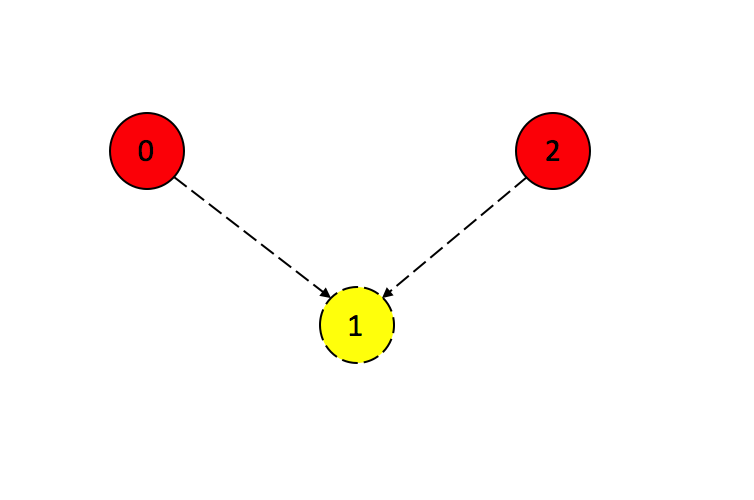
\includegraphics[width=0.6\linewidth]{figures/priority1.png}
			\caption{Solution Using Priority Models}
			\end{figure}
\end{frame}

\subsection{Consistency Models}

\begin{frame}{Consistency Model}
	 \begin{itemize}
	 \item Providing a range of consistency models allows a program to choose the level of
consistency
	 \item This allows the runtime to optimize the parallel execution while maintaining determinism
		\item Full Consistency Model
		 \begin{itemize}
				 \item Executing compute functions must be at least two vertices apart
				 \item Limits the potential parallelism
			 \end{itemize}
		 \end{itemize}
	\let\thefootnote\relax\footnotetext{\tiny[Low et. al., "Distributed GraphLab:A Framework for Machine Learning and Data Mining in the Cloud", VLDB, Vol. 5 No 8, 2012.]}
	 \end{frame}

	 \begin{frame}{Consistency Model}
	 	 \begin{itemize}
			 \item Edge Consistency Model
			 \begin{itemize}
				 \item Ensures each compute function has exclusive read-write access to its
vertex and adjacent edges
				 \item Has read only access to adjacent vertices
				 \item Increases potential parallelism
			 \end{itemize}
					 \item Vertex Consistency Model
			 \begin{itemize}
				 \item Ensures each compute function has exclusive write access to its
vertex and read access to adjacent edges
				 \item Provides maximum parallelism
			 \end{itemize}
		 \end{itemize}
	\let\thefootnote\relax\footnotetext{\tiny[Low et. al., "Distributed GraphLab:A Framework for Machine Learning and Data Mining in the Cloud", VLDB, Vol. 5 No 8, 2012.]}
	 \end{frame}

\begin{frame}{K-Clustering}
	Conflict in k-clustering algorithm
			\begin{figure}
			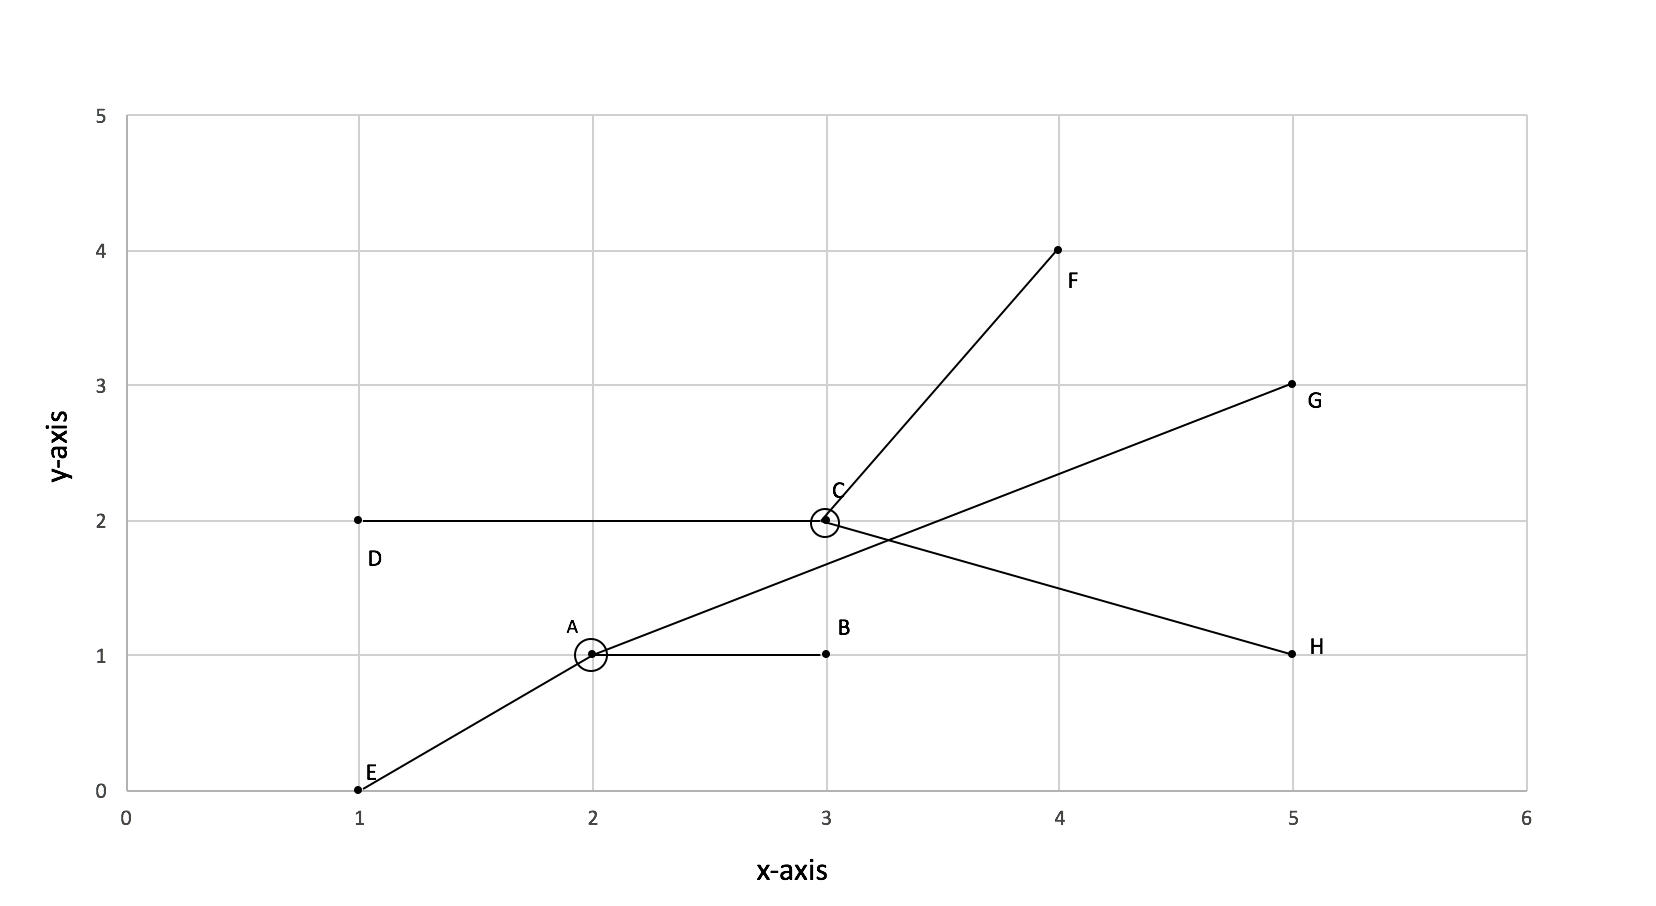
\includegraphics[width=0.8\linewidth]{figures/kcluster1.jpg}
			\caption{Solution Using Consistency Models}
			\end{figure}
\end{frame}

\begin{frame}{K-Clustering}
  Calculating Euclidean distance from each object to both of the clusters:\\
  $DA$=$\sqrt{{(1-2)}^2+{(2-1)}^2}=\sqrt{2}$,
  $DC$=$\sqrt{{(1-3)}^2+{(2-2)}^2}=2$\\
  $\therefore DA<DC$\\
  $BA$ = $\sqrt{{(3-2)}^2+{(1-1)}^2}=1$,
  $BC$ = $\sqrt{{(3-3)}^2+{(2-1)}^2}=1$\\
  $\therefore BA=BC$\\
  $EA$=$\sqrt{{(2-1)}^2+{(1-0)}^2}=\sqrt{2}$,
  $EC$=$\sqrt{{(3-1)}^2+{(2-0)}^2}=\sqrt{8}$\\
  $\therefore EA<EC$\\
\end{frame}

\begin{frame}{K-Clustering}
  $FA$=$\sqrt{{(4-2)}^2+{(4-1)}^2}=\sqrt{13}$,
  $FC$=$\sqrt{{(4-3)}^2+{(4-2)}^2}=\sqrt{5}$\\
  $\therefore FC<FA$\\
  $GA$=$\sqrt{{(5-2)}^2+{(3-1)}^2}=\sqrt{13}$,$GC$=$\sqrt{{(5-3)}^2+{(3-2)}^2}=\sqrt{5}$\\
  $\therefore GC<GA$\\
  $HA$=$\sqrt{{(5-2)}^2+{(1-1)}^2}=3$,
  $HC$=$\sqrt{{(5-3)}^2+{(1-2)}^2}=\sqrt{5}$\\
  $\therefore HC<HA$\\
\end{frame}

\begin{frame}{K-Clustering}
	Conflict in k-clustering algorithm
			\begin{figure}
			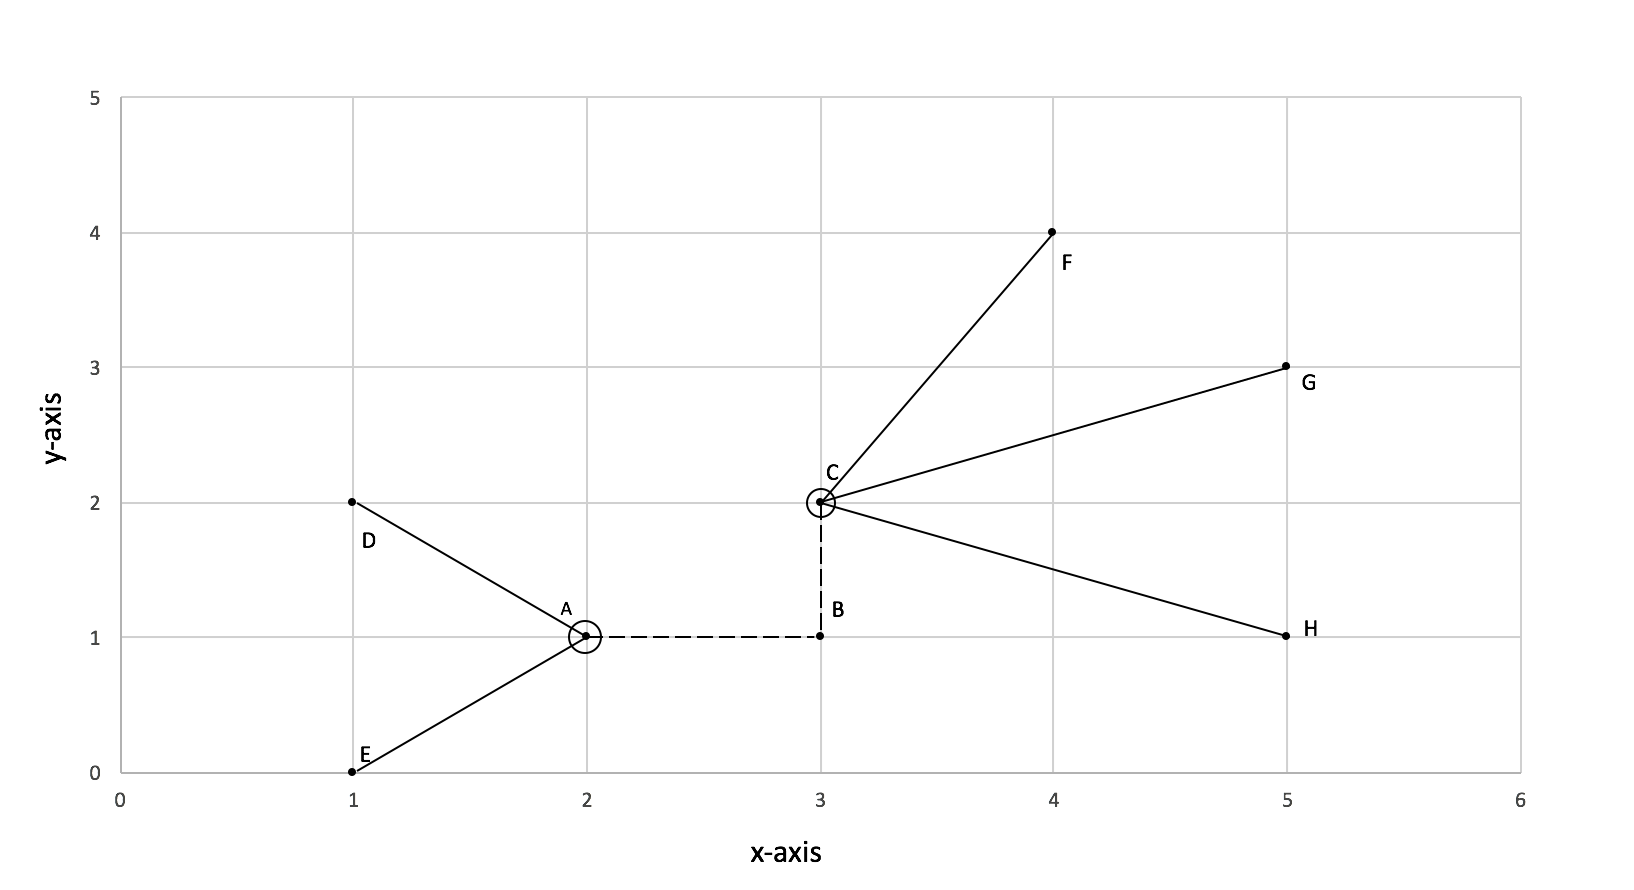
\includegraphics[width=0.8\linewidth]{figures/kcluster2.jpg}
			\caption{Solution Using Consistency Models}
			\end{figure}
\end{frame}

\begin{frame}{K-Clustering}
	Conflict in k-clustering algorithm
			\begin{figure}
			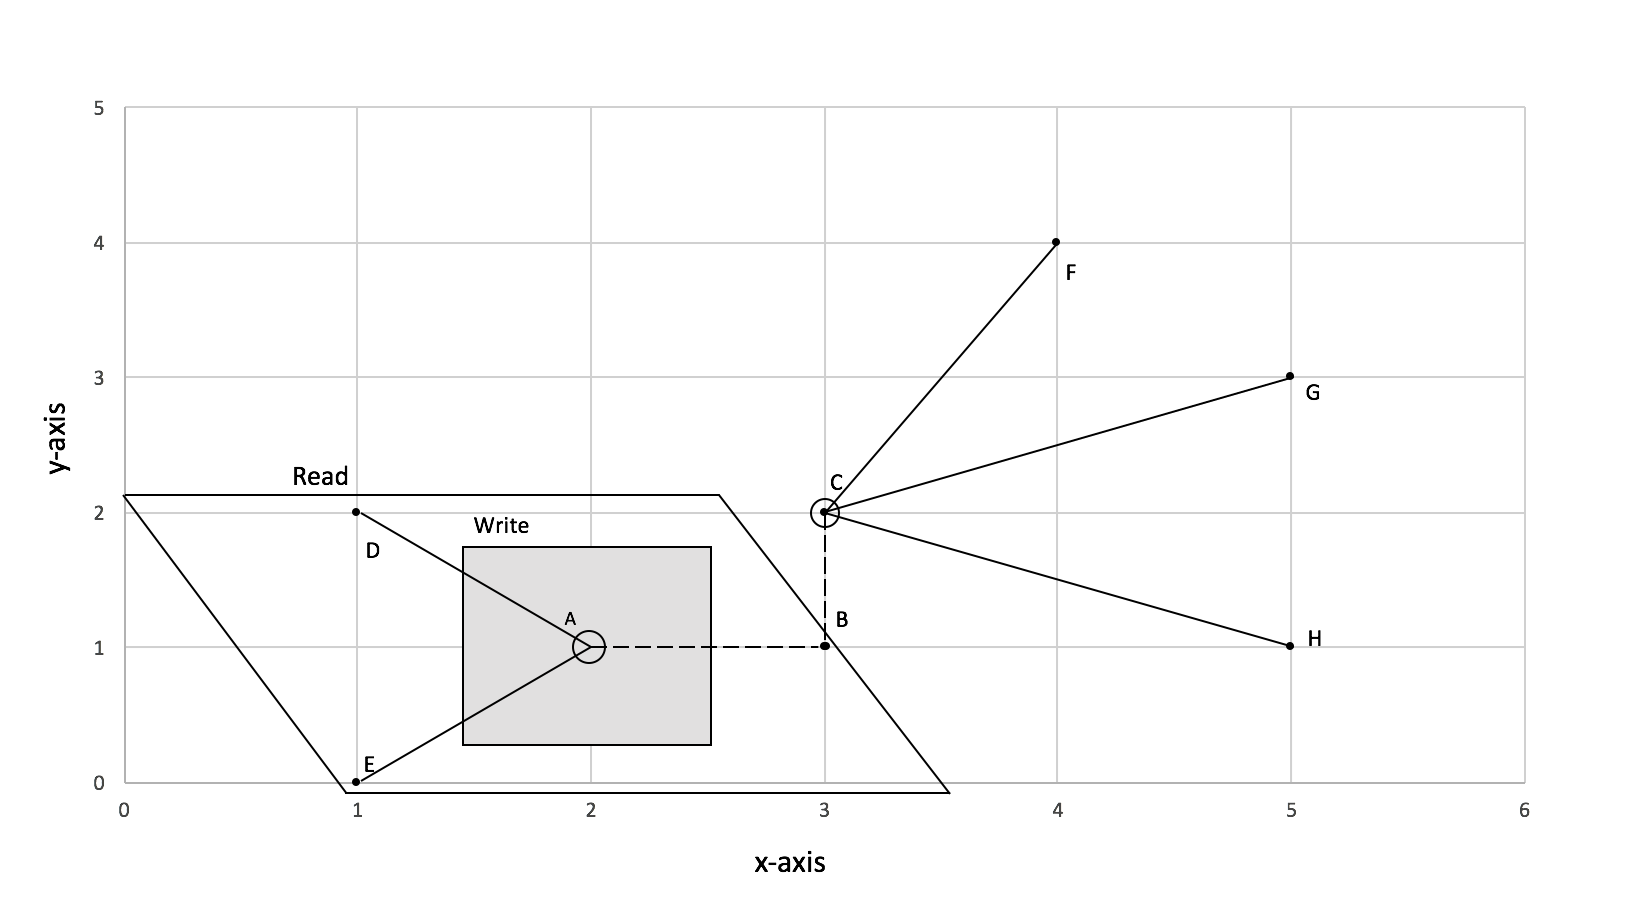
\includegraphics[width=0.8\linewidth]{figures/kcluster3.png}
			\caption{Solution Using Consistency Models}
			\end{figure}
\end{frame}


\begin{frame}
	Conflict in dangling edge
			\begin{figure}
			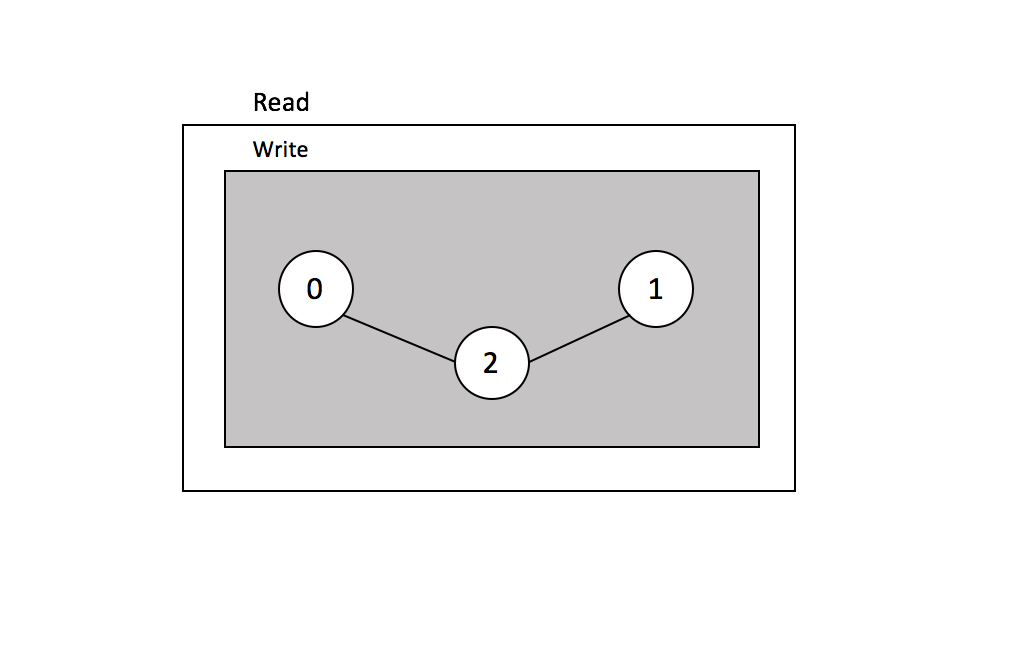
\includegraphics[width=0.6\linewidth]{figures/vnode1.png}
			\caption{Solution Using Consistency Models}
			\end{figure}
\end{frame}
